\documentclass{beamer}

\usepackage{beamerthemesplit}
\usepackage{graphicx}
\usepackage{multicol}
\newcounter{saveenumi}
\newcommand{\seti}{\setcounter{saveenumi}{\value{enumi}}}
\newcommand{\conti}{\setcounter{enumi}{\value{saveenumi}}}

\newcommand{\cram}{Cram\'{e}r-von Mises }
\newcommand{\dis}{distribution }
\newcommand{\vMds}{von Mises
distributions }

 \newcommand{\kronecker}{\raisebox{1pt}{\ensuremath{\:\otimes\:}}} 




\begin{document}





%\frame{\tableofcontents}
%\subsection{Overview of the Circular Data}
\frame
{
  \frametitle{Introduction.}

\begin{itemize}
\item
This paper proposes a new method to test fit of an unobserved (latent) variable 
to a given distribution based on an observed variable and the connection between the two. 
\item
This is largely an unexplored area of Statistics. Here Bayesian 
principles are borrowed to generate the test procedure. 
\item
By choosing an appropriate prior, this procedure yields the \cram 
 or the Anderson Darling  as test statistics. 

\item 
The test has good power against many alternative                                    
densities. Power study results are available upon request.

\item
The procedure was motivated by a paper by Krumbien (1935) and Krumbein's data will be used to give the first (simple) illustration. 

\item 
For a modern example, a test will be applied to test the distribution of the \textcolor{red} {frailty term}
 in a survival analysis  model. Shih and Louis (1995) showed that different frailty distribution induce quite different dependence and therefore 
testing frailty distribution is necessary.
  
 
%\item
%A third example is to test the 
%\textcolor{red} {random effect} in a logistic regression model.  %The cross-sections are 
 %measured by randomly slice through the 
 %whole clay which then randomly slice through the  
%spheres that are in the clay.
\end{itemize} 

}




 \frame
{
  \frametitle{Theory of the Test}
\begin{itemize}
\item 
Observed variables:$\it{x} = [x_1,\cdots, x_n]^{'}$
\item
Unobserved variables: $\it{r} =[r_1,\cdots,r_n]^{'}$ 
\item
\textcolor{red}{$H_o: \it{r}$ follows 
density $g(\it{r}| \theta)$,} with cdf
$G(\it{r}| \theta)$;
prior for parameter $\theta$ is $\pi(\theta)$.

\item
 \textcolor{red}{$H_A$: 
 Alternative density for $r$:
 %\it{r}$ follows
 $g(\it{r}| \theta) \Lambda(\it{r}| \theta)$,}
 where $\Lambda(\it{r}| \theta)$ is a prior distribution to 
  model departure  from the null distribution.

\item  The Prior density $\Lambda(\it{r}| \theta)$ provides a set of possible alternative
distributions that form an alternative band around the null density
\item
Conditional density 
   of $x$ given $r$: 
$h(x|r)$. 
\item 
 The null density of $x$ is 
  \begin{equation*}
  f_o(\it{x}) = \int_{\it{r}} \int_{\theta} 
  h(\it{x}|\it{r})g(\it{r}| \theta)\pi(\theta) 
  d\theta d\it{r}.
  \end{equation*}
  %But $f_o(\it{x}, \it{r}, \theta) = 
  %h(\it{x}|\it{r})g(\it{r}| \theta)\pi(\theta)$
 %and  the alternative density is from 
\end{itemize}
}


 \frame
{
  \frametitle{ The alternative density $f_A(\it{x})$}
 \begin{eqnarray}
  f_A(\it{x})  
  &=& \int_{\it{r}} 
  \int_{\theta} \int_{\Lambda}
  h(\it{x}|\it{r})g(\it{r}| \theta)
  \Lambda(\it{r}| \theta)\pi(\theta) 
  d\Lambda d\theta d\it{r}\nonumber \\
   &=&  \int_{\it{r}} \int_{\theta} 
   f(\it{r}, \it{x}, \theta) 
  \int_{\Lambda}\Lambda(\it{r}| \theta)
  d\Lambda d\theta d\it{r} \nonumber \\
 &=&  f_o(\it{x})  \int_{\it{r}} 
 \int_{\theta} f(\it{r}, \theta| \it{x}) 
 \int_{\Lambda} \Lambda(\it{r}| \theta)
 d\Lambda d\theta d\it{r} \nonumber \\
  &=&  f_o(\it{x})  
  E \left[\int_{\Lambda}\Lambda(\it{r}| \theta)
   d\Lambda|\it{x}\right], \nonumber
\end{eqnarray}

\begin{itemize}
\item The \textcolor{red}{Neyman-Pearson Lemma} 
shows the  likelihood ratio (LR) will maximize power 
subject to level 
$\alpha$.

\item
The LR test statistic is 
$ f_A(\it{x})/ f_o(\it{x})= 
 E\left[\int_{\Lambda}\Lambda(\it{r}| \theta) d\Lambda|\it{x}\right]$
 
\item
Rejection Region:
$C= \{\it{x} | E[\int_{\Lambda}
\Lambda(\it{r}| \theta)d\Lambda |\it{x}] > k\}$;
when under ${H_o},$
Prob[$ \it{x} \in C]=\alpha$.
\end{itemize}
}


 \frame
{
  \frametitle{Define prior density $\Lambda(\it{r}, \theta)$ }
\begin{itemize}
\item Sun and Lockhart (2018) suggest one possibility is 
$$ \Lambda(\it{r}| \theta) = 
\exp \left\{ \epsilon \sum_{i=1}^n
Z(u_i)\right\}/\left[\int_0^1\exp\{\epsilon Z(t) \}dt\right]^n,  $$
where $u_i=G(r_i; \theta),$ the Probability Integral Transformation 
of $r_i$ under the $H_0$   

\item
$Z(t)$ is a \textcolor{red}{Gaussian Process} with 
$E\{Z(t)\}=0$, $0<t<1$
and covariance function $\rho(s,t),$ 
and $\epsilon$ determines 
how far $H_A$ departs from $H_o$. 
% \begin{eqnarray}
 % [\int_0^1\exp\{\epsilon Z(t) \}dt]^n  &=&
  %   [\int_0^1 1+\epsilon Z(t) + \epsilon^2 Z(t)^2/2+\cdots dt ]^n   \nonumber \\
   %   &\approx&
    % [ 1+ \int_0^1\epsilon^2 Z(t)^2/2dt]^n   \nonumber \\
    % &\approx&
     %\exp \{n\epsilon^2 \int_0^1Z(t)^2dt/2. \} \nonumber
 %\end{eqnarray}
 \item
  Classically, the Gaussian Process may be written 
$Z(t)=\sum_j^\infty w_j \sqrt{\lambda_j} g_j(t)$
where $w_j$ are iid $N(0,1)$ 
and  
$\lambda_j$, $g_j(t)$ are eigenvalues and 
eigenfunctions of 
\begin{equation*}
\label{inteq}
\int_0^1 \rho(s,t)g_j(t)dt=\lambda_j g_j(s).
\end{equation*}

\end{itemize}
}



 \frame
{
  \frametitle{Test Statistic with the Gaussian Prior}
  
   Then the test statistic
becomes 

\begin{equation} 
\label{bayes1}
\textcolor{red}{S=E\left( \exp\left\{ \sum_{j=1}^{\infty}
\frac{\epsilon^2 \lambda_j 
[\sum_{i=1}^n g_j(u_i)]^2}
     {2(n\epsilon^2\lambda_j+1)} \right\}\Bigg|\it{x}\right).}
\end{equation}


 when $\rho(s,t)=min(s,t)-st$, $\lambda_j=1/(\pi^2j^2)$  
and $g_j(s)= \sqrt{2}\cos(\pi js)$, $S$ is the average
 \cram $W^2$. 
 Figure 1 and 2: comparisons of Null and Alter. densities.
 \begin{center}
%\begin{figure}
 %\label{f1}
 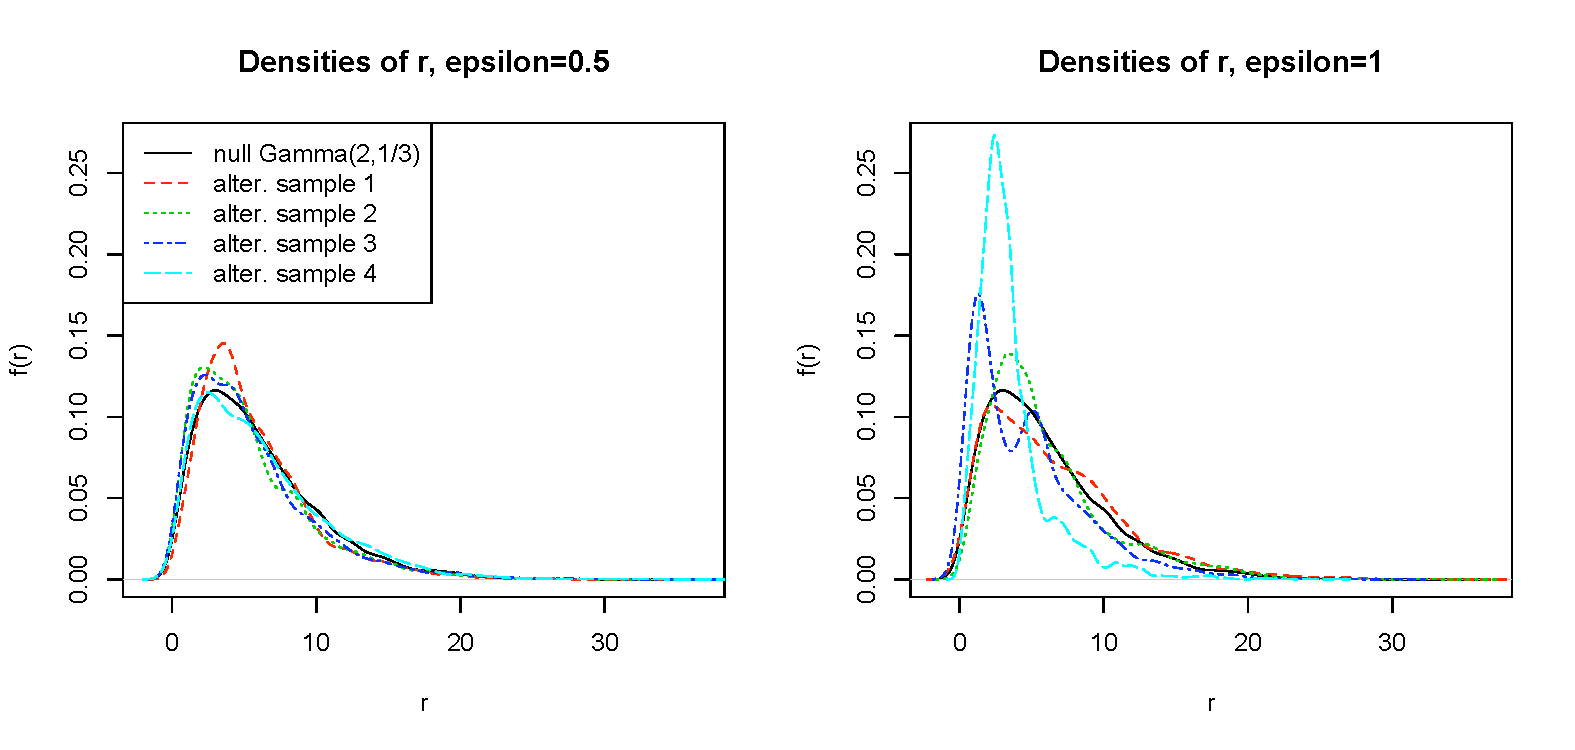
\includegraphics[width=20em]{guassplot.pdf}
 %\end{figure}
 \end{center}

 }
 

 
 \frame
{
  \frametitle{Test Procedures}
  
  
 For statistic $S$, % the average $W^2$,  
 the posterior joint density of $r$ and $\theta$
 must be found by Gibbs sampling. 
%headings: test procedure. 
The steps are as follows:
\begin{enumerate} 
\item
Assign prior distributions for 
%the unknown parameters 
$\theta$ in $g(x|\theta)$. 
\item
Sample from 
%the posterior density 
$f(r, \theta|x)$ by the Gibbs sampling algorithm:
sample iteratively from 
the full conditionals:  \\
(a) $f(r_i |r^*, \theta, x), \; i=1, \cdots, n$
where $r^*$ denotes the set of $r$ 
omitting $r_i$, this gives $n$ new 
values of $r$ for a given $\theta$\\
(b) $f(\theta |r , x)$. 
\item
Compute $S$ in (\ref{bayes1}) using
% the realizations of 
the $[r, \theta]$ generated from 
 the previous step (after a burn-in period), 
 this is the test statistic $S^*$ based on the 
 given $x$ values.
 \item
 To obtain the distribution of $S$,
 bootstrap a set of $\bold{r}$ from 
 the null distribution, using 
 an estimate of $\theta$: this may be
 the posterior modes in step 2 or 
 the EM algorithm estimate
 or some other efficient estimates 
 \end{enumerate}
}



 \frame
{
  \frametitle{Test Procedures}
  Steps continue...
\begin{itemize}
\item[5]
 Generate 
a set of $\bold{x}$ from $h(x|\bold{r})$. 
\item[6]
Calculate 
the statistic $S$, call it $S_d$. 



\item[7]
Repeat Steps $4-6$  $M$ times, say 100, 
to get 
$M$ values of $S_d$; these give 
an estimated 
distribution of $S$ under $H_o$.
\item[8]
Hence calculate the 
$p$-value of $S^*$.
\end{itemize}

Example 1: Krumbein (1953) studied a dataset of spherical rocks. 
 The data observed, $x$, are the radii of circular
 cross-sections of the rocks from random slicing. 
 The variable of interest is the radii ($r$) of the rocks, which 
embedded in sediments and therefore are unobserved.
 %The cross-sections are 
 %measured by randomly slice through the 
 %whole clay which then randomly slice through the  
%spheres that are in the clay. 
% \vspace{0.1cm}
% \begin{center}
%%\begin{figure}
% %\label{f1}
% 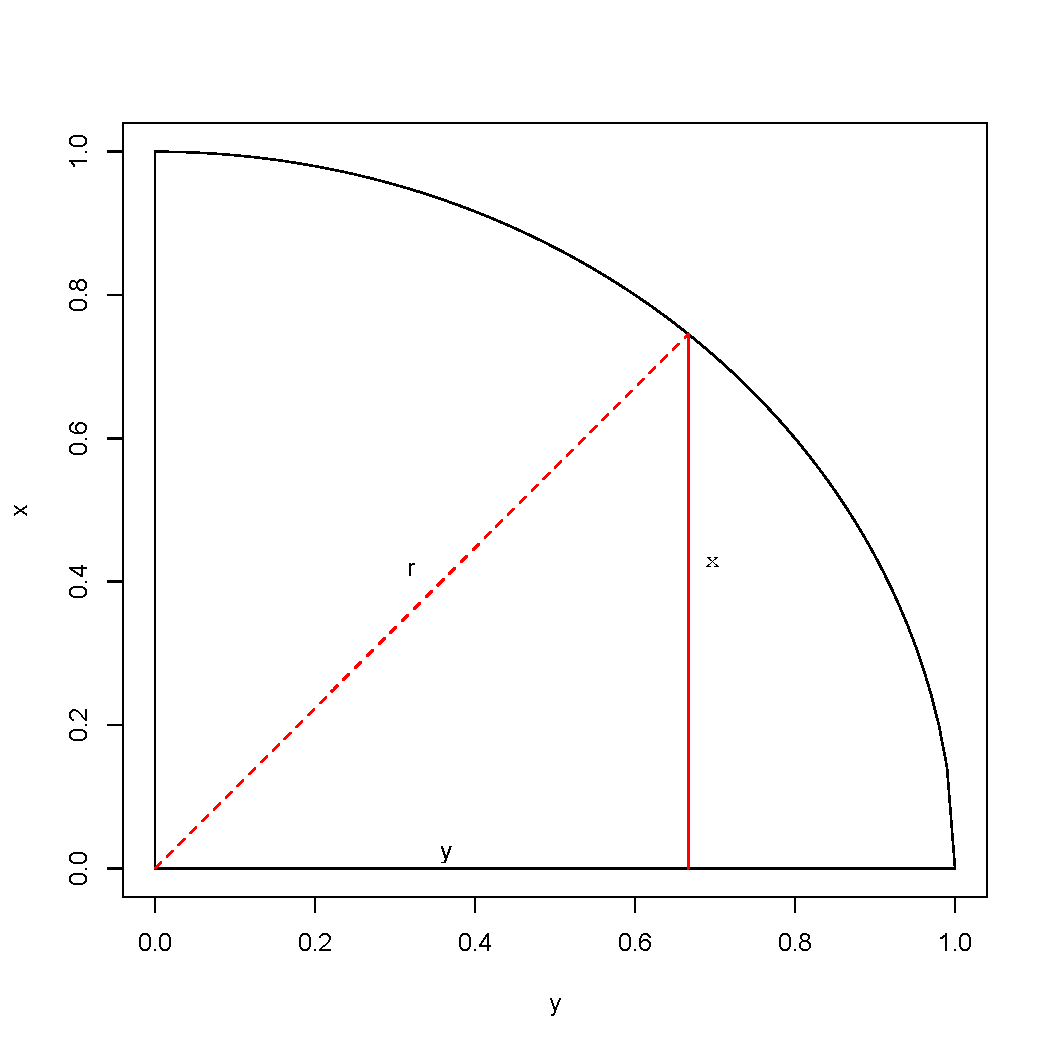
\includegraphics[width=10em]{krum1signed.pdf}
% %\end{figure}
% \end{center}
% \vspace{0.1cm}
% \end{multicols}
% \vspace{0.1cm}
%\textbf{Table: Number of sandstone  in given intervals.}
%\begin{center}
%\begin{tabular}{ccccccccccc}
%\hline
%\multicolumn{10}{c}{cell midpoint(in mm)}\\
%\hline
%&06&10&13&16&20&24&28
%&32&36&40\\
%\hline
%$x$&43&79&93&70&27&16&9&5&1&0\\
%$r$&2&22&89&72&57&35&28&23&10&4\\%wrong
%\hline
%\end{tabular}
%\end{center}
Researchers wanted to test if the radii of the rocks follow a Gamma distribution, so the null hypothesis is
$H_0: \bold{r} \sim $ Gamma ($\alpha, \beta$). 
The above steps become
 \vspace{-0.2cm}
 \begin{enumerate}
\item
Choose a conjugate prior density for $\alpha$ and $\beta$:
 \begin{equation*}
 \pi(\alpha, \beta| v, q, s, t)\propto \frac{v^{\alpha-1}e^{-q/\beta}}
 {\Gamma(\alpha)^t\beta^{\alpha s}}.
  \end{equation*}

 \seti
 \end{enumerate}
}
  
  
 
    \frame
{
  \frametitle{Krumbein's Example.}
 \begin{enumerate}
 \conti
\item
A Gibbs sampler scheme is used which alternates among $\bold{r}, \alpha$, 
  and $\beta$ , the full conditionals for 
  $p(r_i, \alpha, \beta| x_i, v, q, s, t):$
   %%%%ZHENG change p to v.
   \begin{equation*}
   \label{cond_r}
 p(r_i| x_i, \alpha, \beta)\propto 
  \frac{r_i^{\alpha-2}e^{-r_i/\beta}}{\sqrt{r_i^2-x_i^2}},
  \end{equation*}
   \begin{equation*}
    \label{cond_alpha}
 \pi(\alpha|\bold{r})\propto 
 \frac{(p\prod_{i=1}^nr_i/\beta^{(n+s)})^{\alpha}}{\Gamma(\alpha)^{n+t}},
  \end{equation*}

   \begin{equation*}
    \label{cond_beta}
 \pi(\beta|\bold{r})\propto 
 e^{-(q+\sum_{i=1}^nr_i)/\beta}
\beta^{-\alpha (n+s)}.
  \end{equation*}
 

\item
Calculate $S=0.199$  in equation (\ref{bayes1}).
%see the trace plots for 
%$\alpha$ and $\beta$. 
%\seti
\item
The EM algorithm is used to estimate $\alpha$ and $\beta,$ 
$$L=  \prod_{i=1}^n x_i/(\Gamma(\alpha)\beta^\alpha)
\int_{x_i}^\infty \frac{r_i^{\alpha-2}\exp(-r/\beta)}
{\sqrt{r_i^2-x_i^2}}dr_i; 
$$ 
\item
The p value is 0.043.
Gamma is rejected at the $5\%$ level.
\end{enumerate}
}

  




  
 
 \frame
{
 \frametitle{ Testing a Frailty Term.}
 
McGilchrist and Aisbett (1991)
 give time to first and second 
 recurrence of kidney infection 
 in 38 patients on dialysis.
 \begin{itemize}
 \item Let $y_{ij}$ be the observed times 
and $\delta_{ij}$ be the indicator
$(\delta_{ij}=1$, if event for patient $i$, 
 recurrence $j$ occurred;   
$\delta_{ij}=0$, right censored)
 for $i=1,\cdots, 38$
and $j=1,2$.
\item
 With the Proportional Hazards (PH) model, the 
likelihood contribution 
of the $i$th patient in 
the $j$th recurrence  is (conditional 
on $w_i$): \\
%\begin{equation*}
$L_{ij}=\{h_0(y_{ij})w_i
\exp{(\mu_{ij})}\}^{\delta_{ij}}
\exp\{-H_0(y_{ij})w_i\exp{(\mu_{ij})}\}. $
%\end{equation*} 
\item Assume the baseline hazard to be 
a Weibull density:
$h_0(y_{ij})=\lambda \rho y_{ij}^{\rho-1}$ 
and $H_0(y_{ij})=\lambda 
y_{ij}^\rho$ .
\item Let
$\mu_{ij}$ be a linear function of 5 covariates;  
%$\mu_{ij} = \beta_1 AGE_{ij}
%+\beta_2 SEX_{i} +\beta_3 DISEASE_{i1}
%+\beta_4 DISEASE_{i2} +\beta_5 DISEASE_{i3}$. 
$AGE_{ij}$, 
%is a continuous covariate,  
$SEX_{i}$ and
%is a dichotomous covariate,
$DISEASE_{ik}$, for $k=1,2,3$ - 
%dummy variables representing 
%the difference between a baseline disease 
%and 3 others.
 representing 
4 different 
diseases. 
\item
Finally, the model includes a random effect (frailty term)
 $w_i$ for 
 patient $i$.
 \end{itemize}

}


 \frame
{
  \frametitle{Example: Testing a Frailty Term.}

The null is $Ho: w_i \sim$ lognormal$(0, \tau)$.
\begin{enumerate}
\item Assign 
%In step 2 above, the regression coefficients and the precision of the 
%random effect  are given 
``non-informative"
priors.
% each $\lambda,$ and $\beta_l, \; l=1, \cdots, 5 \sim
 % N(0, 10000)$  
%and $\tau\sim$ Gamma($0.0001$, $0.0001$).
%The shape parameter $\rho$ of the Weibull density 
 %is assigned a Gamma(1, 0.0001) prior.

\item
To sample from the full conditionals of 
$\pi(w_i, \beta_h, \rho, \lambda, \sigma^2|y_{ij}, \delta_{ij})$, 
the block updating strategies 
 and
the Metropolis algorithm within Gibbs are employed.  
 \item
 %after the first 1000 samples 
 %(burn in period), 9000 posterior 
%samples were used to 
The value $S^*$ in (\ref{bayes1}) is 
$S^*= 0.165$.
%The mean of these samples are
%$\tilde{\lambda}=-4.7$, $\tilde{\beta1}=-2.0$,  $\tilde{\beta2}=0.003$, 
%$\tilde{\beta3}=0.1$, $\tilde{\beta4}=0.6$, $\tilde{\beta5}=-0.9$ 
%$\tilde{\rho}=1.2$ and $\tilde{\sigma}=0.7$.
%The value 0.165$. 
\item
The R package ``parfm" is used to 
estimate $\beta$s, $\rho$, $\lambda$, $\sigma^2$. 
%which maximizes the marginal likelihood. 
%by integrating out the frailty parameter. 
%$\hat{\lambda}=-4.34$, $\hat{\beta1}=-1.88$,  $\hat{\beta2}=0.003$, 
%$\hat{\beta3}=0.12$, $\hat{\beta4}=0.61$, $\hat{\beta5}=-1.14$ 
%$\hat{\rho}=1.16$ and $\hat{\sigma}=0.56$.
%The estimates are very close to the posterior means obtained in
%step 4. 
Using these
estimates, bootstrap samples 
were generated using the 
algorithm 7.3 by Davison 
and Hinkley (1997) and hence the distribution of $S$.
%%To check the bootstrap samples, we refitted the  
%%model to each of the bootstrap samples.
%The means of the estimates are 
%$\hat{\lambda}_{boot}= -4.14, 
%\hat{\beta_1}_{boot}=-1.97,
%\hat{\beta_2}_{boot}= 0.003,
%\hat{\beta_3}_{boot}=0.13,
%\hat{\beta_4}_{boot}=0.61,
%\hat{\beta_5}_{boot}=-1.14,
 %\hat{\rho}_{boot}=1.22$ and $\hat{\sigma}_{boot}=0.49$.
\item
%The means of estimates are very close to the original estimates.
The p-value of $S$ is 
 0.86 and a lognormal distribution
 for the frailty is not rejected. 
 \end{enumerate}
 }
  
  
% \frame
%{
%  \frametitle{Summary}
%  \begin{itemize}
%\item
%Bayesian methods are used with Neyman Pearson theory to test the distribution
%of a latent variable. This variable $r$ is related to an observed variable $x$.
%
%\item
%From NP theory,  the LR test statistic is the statistic of choice, by suitable choice 
%of prior, the LR statistic becomes the expectation of \cram $W^2$. This 
%expectation is estimated as follows:
%\item
%The join density of $x$ and $r$ and hence the conditional density 
%of $r|x$ can be found.
%\item 
%From this density, 
% many $r$ samples are drawn and for each sample a test statistic, e.g. $W^2$,
% is calculated.
% \item 
% The final test statistic is the average of these.
%\item
%At present, the distribution of the test statistic is found by Monte Carlo.
%\item 
%Power study results show the test is powerful against a wide range of alternative distributions; the results are available upon request.
%\end{itemize}
%}

%
% \frame
%{
%  \frametitle{References}
% 
%  \begin{itemize}
%
%\item
%Davison, A.C. \& Hinkley, D.V. (1997), Bootstrap Methods and Their Application. \textit{Cambridge University Press}.
%
%\item
%Krumbein, W. C. (1935), 
%Thin-Section Mechanical Analysis of Indurated Sediments. 
%\textit{Journal
%of Geology}, 43, 482-496.
%
%\item
%Sun and Lockhart (2018),
%Bayesian optimality for  Beran's class of tests of uniformity around the circle, \textit{Journal of Statistical Planning and Inference}, 
%DOI information: 10.1016/j.jspi.2018.03.006 
%
%%\item
%%McGilchrist, C. A., Aisbett, C. W. (1991),
%%Regression with Frailty in Survival Analysis. 
%%\textit{Biometrics}, 42, 461-466.
%
%\item
%Shih, J. H. and Louis, T. A. (1995). Inference on the association 
%parameter in copula models for bivariate survival data. \textit{Biometrics},
%51, 205-220.
%\end{itemize}
%  
%  
%  }
  
\end{document}





  
    
  